\documentclass[a4paper,11pt]{article}

\usepackage{inputenc}
\usepackage[T1]{fontenc}
\usepackage[frenchb]{babel}
\usepackage{fancyhdr,fancybox} % pour personnaliser les en-têtes
\usepackage{lastpage,setspace}
\usepackage{amsfonts,amssymb,amsmath,amsthm,mathrsfs}
\usepackage{relsize,exscale,bbold}
\usepackage{paralist}
\usepackage{xspace,multicol,diagbox,array}
\usepackage{xcolor}
\usepackage{variations}
\usepackage{xypic}
\usepackage{eurosym,stmaryrd}
\usepackage{graphicx}
\usepackage[np]{numprint}
\usepackage{hyperref} 
\usepackage{tikz}
\usepackage{colortbl}
\usepackage{multirow}
\usepackage{MnSymbol,wasysym}
\usepackage[top=1.5cm,bottom=1.5cm,right=1.2cm,left=1.5cm]{geometry}
\usetikzlibrary{calc, arrows, plotmarks, babel,decorations.pathreplacing}
\setstretch{1.25}
%\usepackage{lipsum} %\usepackage{enumitem} %\setlist[enumerate]{itemsep=1mm} bug avec enumerate

\pagestyle{fancy}


\begin{document}
	
\lhead{}\chead{}\rhead{}\lfoot{Ivanhoé Botcazou}\cfoot{\thepage/3}\rfoot{Année~2023-2024 }\renewcommand{\headrulewidth}{0pt}\renewcommand{\footrulewidth}{0.4pt}

\title{Graphiques et types de variables sous les critère de M....}
\maketitle
%variables (nominale, ordonnée et quantitative
\section{Variables quantitatives}

\begin{figure}[h] % Utilisation de l'environnement "figure"
	\centering
	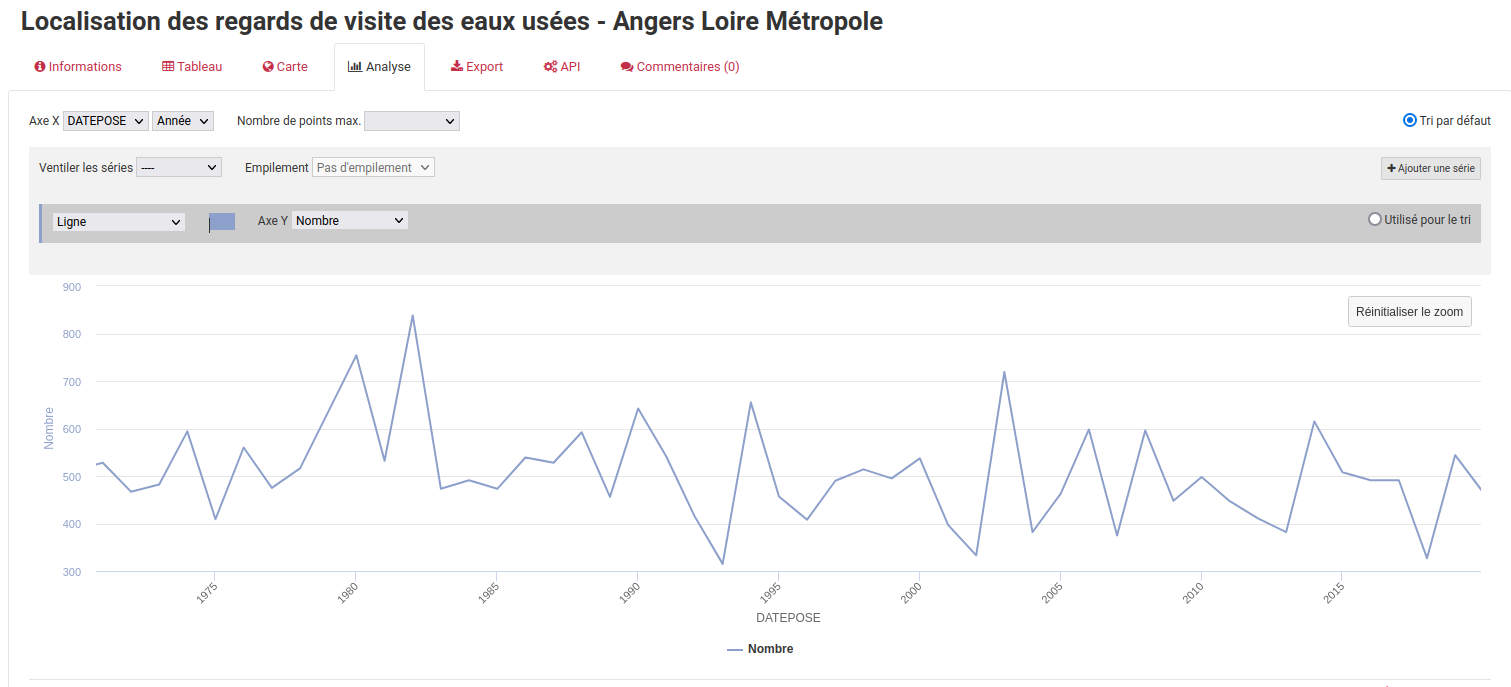
\includegraphics[width=0.7\linewidth]{quantitatif_ok.png} % Inclut l'image
	\caption{Good quantitatif graph } % Ajoute une légende sous l'image
	\label{fig1}\hfil\\ % Ajoute une étiquette pour référencer l'image dans le texte
	
	
	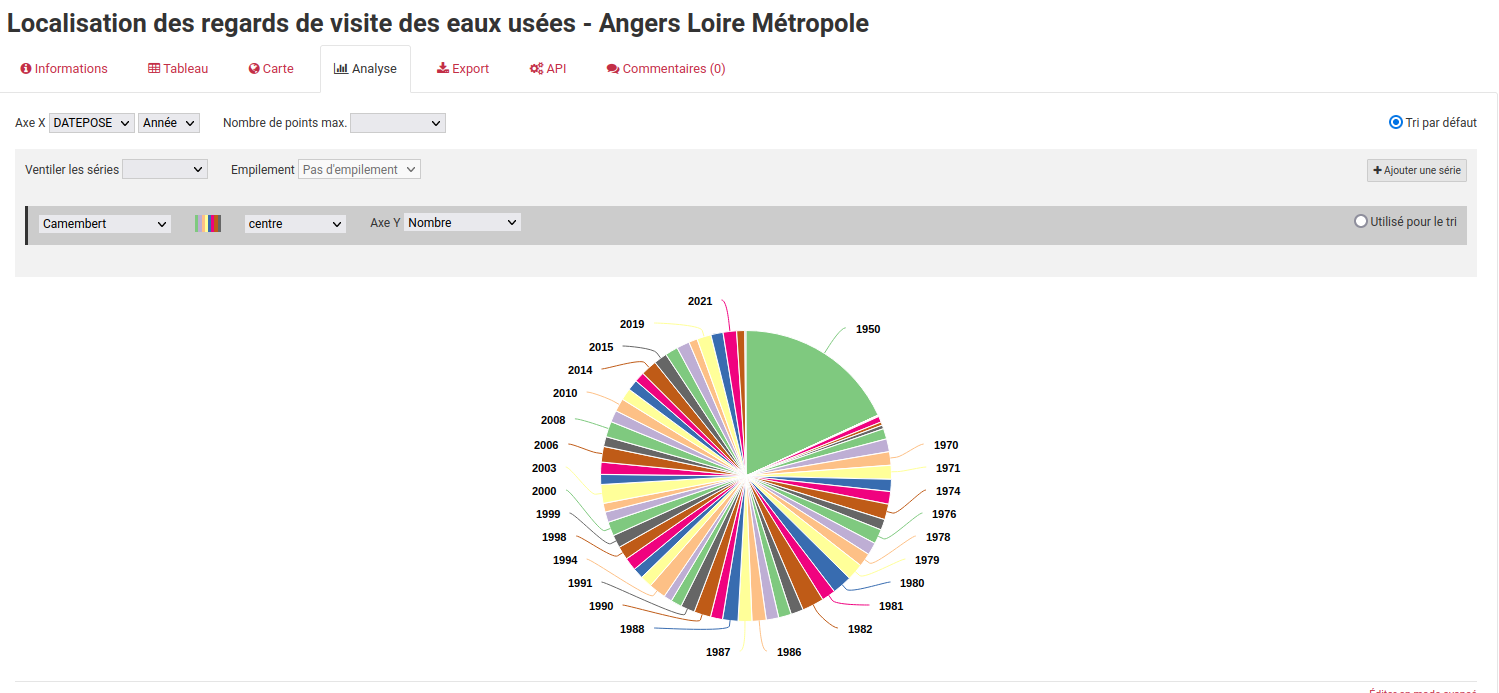
\includegraphics[width=0.8\linewidth]{quantitatif_no.png} % Inclut l'image
	\caption{Bad quantitatif graph } % Ajoute une légende sous l'image
	\label{fig2} % Ajoute une étiquette pour référencer l'image dans le texte
\end{figure}
Nous mettons en opposition ces deux graphiques qui représentent le nombre de regards de visite des eaux usées installées par année dans la ville d'Angers. Grâce aux critères de la combinatoire de Mackinlay nous savons que pour les variables quantitatives, les trois points les plus importants pour un graphique de ce genre sont la position, la longueur et les angles. Le graphique 1 respecte ses règles, la courbe au centre est bien positionnée, les angles décrivent bien les fluctuations au cours du temps. En comparaison, le graphique 2 en secteur ("camembert") n'est pas judicieux, les angles sont trop petits et les couleurs trop nombreuses pour laisser passer de l'information dans les données. 
\newpage

\section{Variables nominales}

\begin{figure}[h] % Utilisation de l'environnement "figure"
	\centering
	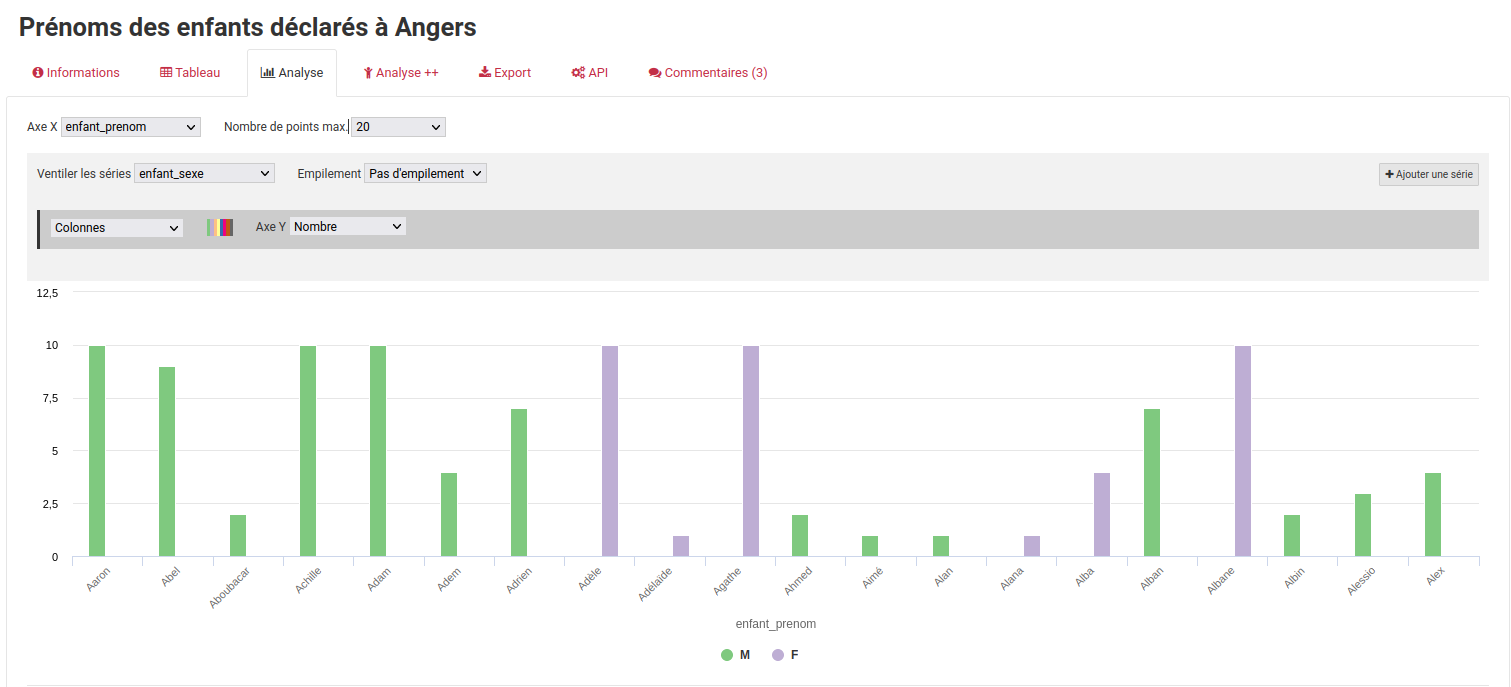
\includegraphics[width=1\linewidth]{nominal_ok.png} % Inclut l'image
\caption{Good nominal graph } % Ajoute une légende sous l'image
	\label{fig3}\hfil\\ % Ajoute une étiquette pour référencer l'image dans le texte
	
	
	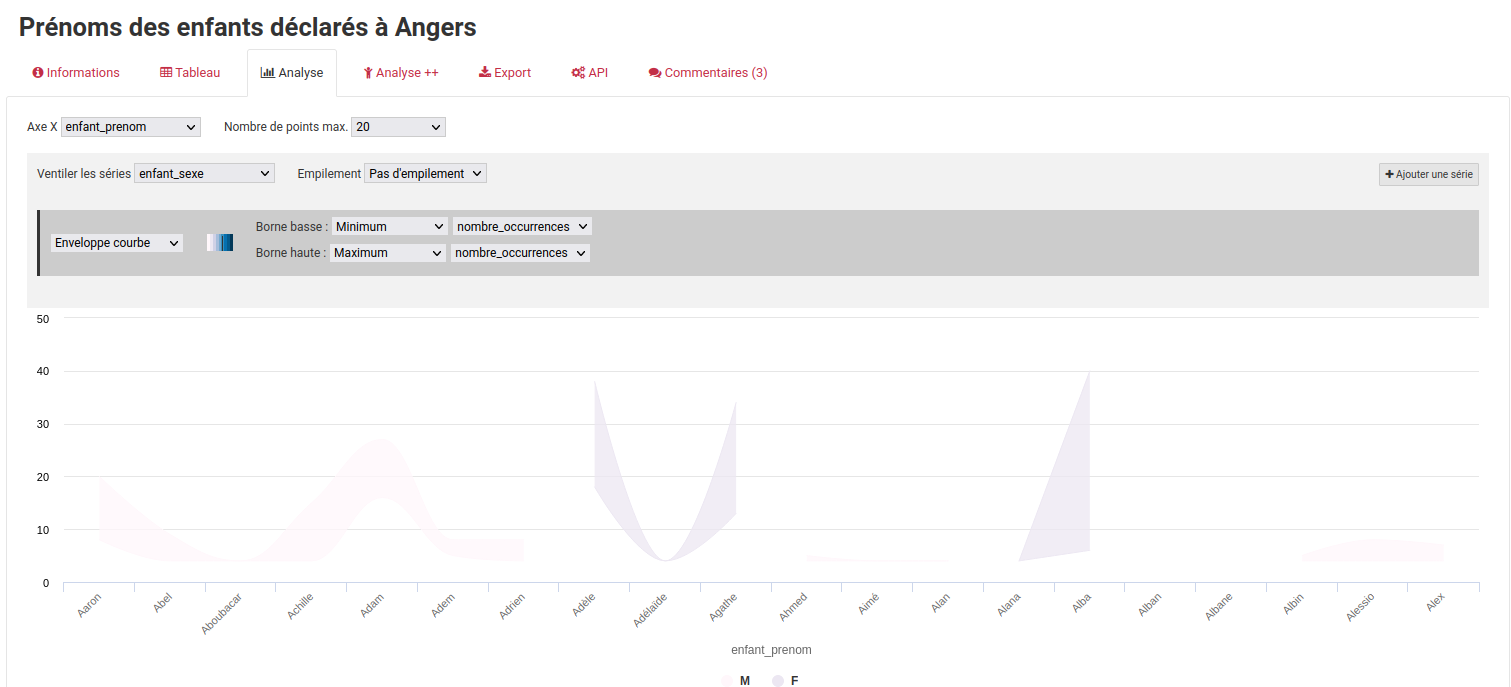
\includegraphics[width=1\linewidth]{nominal_no.png} % Inclut l'image
	\caption{Bad nominal graph } % Ajoute une légende sous l'image
	\label{fig4} % Ajoute une étiquette pour référencer l'image dans le texte
\end{figure}
Nous mettons en opposition ces deux graphiques qui représentent pour 20 prénoms différents, le nombre de personnes nommées ainsi sur une période de 1 an dans la ville d'Angers. Grâce aux critères de la combinatoire de Mackinlay nous savons que pour les variables nominales, les trois points les plus importants pour un graphique de ce genre sont la position, la teinte et la texture. Le graphique 1 respecte ses règles, les différents prénoms sont positionnés sur l'axe des abscisse et la représentation sous forme d'histogramme trouve du sens. La teinte des rectangles nous permets de bien voir la distinction entre les prénoms masculins et les prénoms féminins (Nous pourrions l'accentuer davantage). En comparaison, le graphique 2 sous forme de courbe à moitié remplie ne nous permets pas de comprendre correctement données suivantes. La teinte n'est pas non plus adaptée.

\newpage

\section{Variables ordonnées}

\begin{figure}[h] % Utilisation de l'environnement "figure"
	\centering
	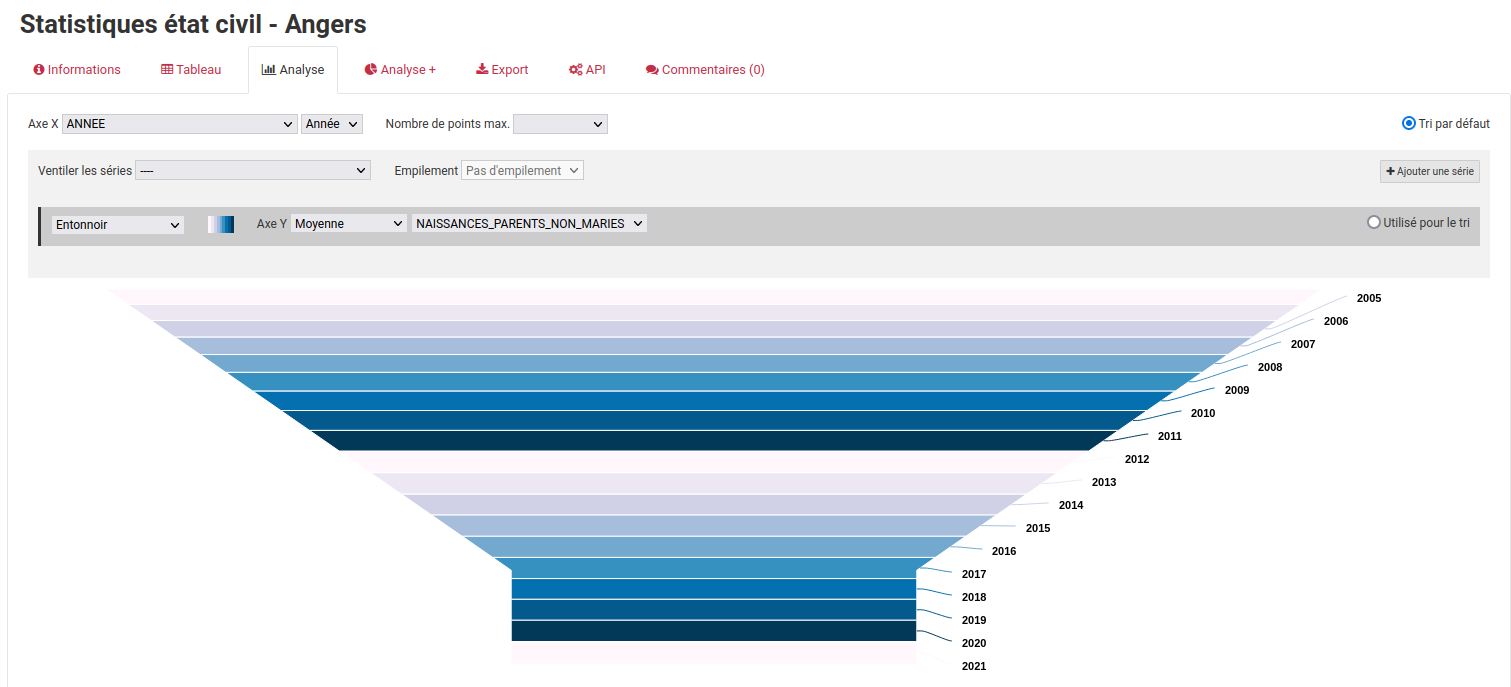
\includegraphics[width=1\linewidth]{ordinal_ok.png} % Inclut l'image
	\caption{Good ordinal graph } % Ajoute une légende sous l'image
	\label{fig5}\hfil\\ % Ajoute une étiquette pour référencer l'image dans le texte
	
	
	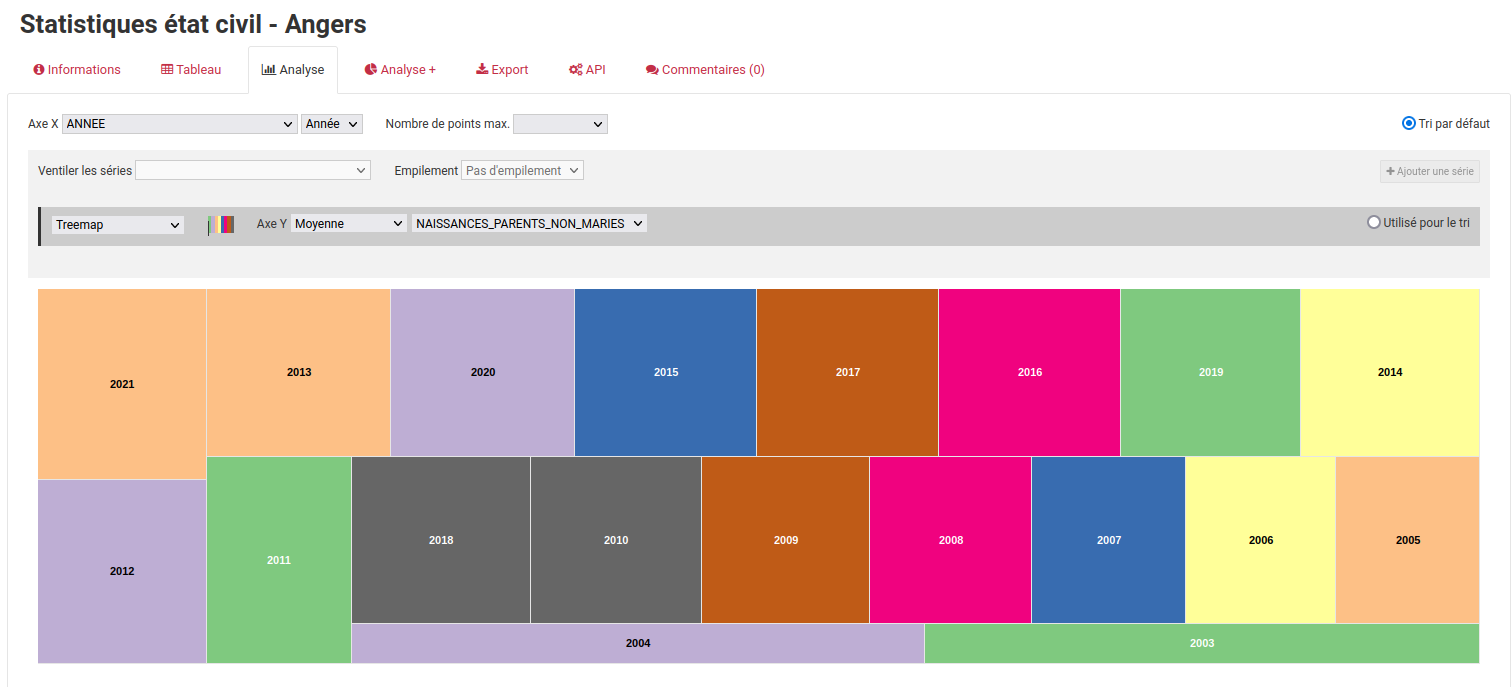
\includegraphics[width=1\linewidth]{ordinal_no.png} % Inclut l'image
	\caption{Bad ordinal graph } % Ajoute une légende sous l'image
	\label{fig6} % Ajoute une étiquette pour référencer l'image dans le texte
\end{figure}

Nous mettons en opposition ces deux graphiques qui représentent les statistiques d'état civil sur des données ordonnées par années dans la ville d'Angers. Grâce aux critères de la combinatoire de Mackinlay nous savons que pour les variables ordonnées, les trois points les plus importants pour un graphique de ce genre sont la position, la densité et la saturation. Le graphique 1 respecte en partie ses règles, les différentes années sont ordonnées à la verticale sous forme d'entonnoir. La densité pourrait être plus accentuée par des des largueurs plus importantes selon les quantités données. La saturation est bien agencée, cependant une échelle de saturation serait appréciable. En comparaison, le graphique 2 sous forme de blocs éparpillés ne reflète plus l'aspect ordonnée des années. La présences des couleurs en trop grande quantité perd le lecteur, c'est une contradiction avec les critères de la combinatoire de Mackinlay.

\newpage

\end{document}




